

\begin{frame}{Variational Autoencoder}
  \begin{itemize}
      
      \item Autoencoder: \begin{itemize}
        \item Encoder $\mathbf{E}:\mathbb{R}^n \rightarrow \mathbb{R}^m$ und Decoder $\mathbf{D}:\mathbb{R}^m \rightarrow \mathbb{R}^n$
        \item Ziel: Eingabedaten komprimieren und anschließend rekonstruieren
        \item Bottleneck - Dimension der Latentrepräsentation kleiner als die Eingabedimension $(m<n)$
        \item diskreter Latentraum
      \end{itemize}
      \item Variational Autoencoder: \begin{itemize}
        \item probabilistischer Ansatz
        \item Datensatz wird durch Wahrscheinlichkeitsfunktion $P(X)$ beschrieben
        \item Encoder speichert Daten als Verteilung im Latentspace $p_\theta (\mathbf{z\mid x})$
        \item Punkte können aus dieser Verteilung gezogen werden $z \sim p_\theta (\mathbf{z\mid x})$
        \item Decoder rekonstruiert Ausgabe aus Latentvektor $z$ mit $p_\theta (\mathbf{x\mid z})$
      \end{itemize}
  \end{itemize}
\end{frame}

\begin{frame}{Variational Autoencoder}
  \begin{figure}
    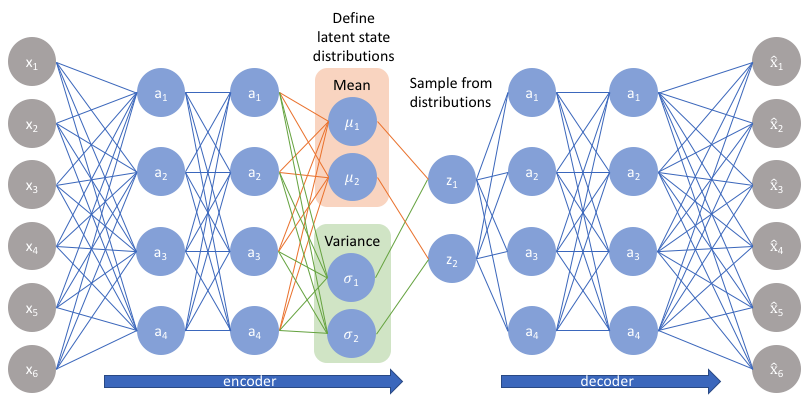
\includegraphics[width=0.7\textwidth]{bilder/vae.png}
    \caption{Variational Autoencoder}
    \end{figure}
\end{frame}

\begin{frame}{Evidence Lower Bound}
  \begin{equation*}
    p_\theta (\mathbf{z\mid x}) = \frac{p_\theta (\mathbf{x\mid z}) p_\theta (\mathbf{z})}{p_\theta(\mathbf{x})}
\end{equation*} nicht berechenbar, deshalb durch Inferenzmodell approximiert $q_\phi (\mathbf{z\mid x}) \approx p_\theta (\mathbf{z\mid x})$.

Optimierungsziel ist Minimierung des Rekonstruktionsfehlers des generativen Modells $\theta$ zwischen Eingabe und Ausgabedaten, sowie Minimierung der Kullback-Leibler-Divergenz  $D_{KL}(q_\phi(\mathbf{z\mid x})\parallel p_\theta(\mathbf{z\mid x}))$.


\end{frame}

\begin{frame}{Evidence Lower Bound}
  Für eine beliebige Wahl der Decoder Parameter $\phi$ gilt:
  \begin{align*}
    log(p_\theta(\mathbf{x})) &= \mathbb{E}_{ q_\phi(\mathbf{z\mid x}) } [log( p_\theta(\mathbf{x}) )] \nonumber \\
    &= \mathbb{E}_{q_\phi( \mathbf{z\mid x} )} \Bigl[ log \Bigl[ \tfrac{ p_\theta(\mathbf{x,z}) }{ p_\theta(\mathbf{z \mid x}) } \Bigr] \Bigr] \nonumber \\
    &= \mathbb{E}_{q_\phi( \mathbf{z\mid x} )} \Bigl[ log \Bigl[ \tfrac{ p_\theta(\mathbf{x,z}) }{ q_\phi( \mathbf{z\mid x} ) } \tfrac{ q_\phi( \mathbf{z\mid x} ) }{ p_\theta(\mathbf{z \mid x}) }\Bigr] \Bigr] \nonumber \\
    &= \underbrace{\mathbb{E}_{q_\phi( \mathbf{z\mid x} )} \Bigl[ log \Bigl[ \tfrac{ p_\theta(\mathbf{x,z}) }{ q_\phi( \mathbf{z\mid x} ) } \Bigr] \Bigr]}_{=\mathcal{L}_{\theta,\phi}(\mathbf{x}) \text{ (ELBO)}} + \underbrace{\mathbb{E}_{q_\phi( \mathbf{z\mid x} )} \Bigl[ log \Bigl[ \tfrac{ q_\phi( \mathbf{z\mid x} ) }{ p_\theta(\mathbf{z \mid x}) }\Bigr] \Bigr]}_{=D_{KL}(q_\phi(\mathbf{z\mid x})\parallel p_\theta(\mathbf{z\mid x}))} 
  \end{align*}
  mit $D_{KL}(q_\phi(\mathbf{z\mid x})\parallel p_\theta(\mathbf{z\mid x})) \geq 0$. Somit lässt sich die Lossfunktion $\mathbf{L}$ aufstellen.
  \begin{align*}
    \mathcal{L}_{\theta,\phi}(\mathbf{x}) &= log(p_\theta(\mathbf{x})) - D_{KL}(q_\phi(\mathbf{z\mid x})\parallel p_\theta(\mathbf{z\mid x})) \leq log(p_\theta(\mathbf{x})) \\
\mathbf{L}_{\theta,\phi} &= -\mathcal{L}_{\theta,\phi}(\mathbf{x}) = -log(p_\theta(\mathbf{x})) + D_{KL}(q_\phi(\mathbf{z\mid x})\parallel p_\theta(\mathbf{z\mid x}))  \\
    \hat{\theta},\hat{\phi} &= \underset{\theta, \phi}{\arg\min \ } \mathbf{L}_{\theta,\phi}
\end{align*}
\end{frame}

\begin{frame}{Reparametisierung}
  Samplen von $z \sim q_\phi(\mathbf{z\mid x})$ ist nicht deterministisch $\Rightarrow$ keine Backpropagation durchführbar,
  deshalb mittels Reparametisierung $z$ durch deterministische Funktion $f_\phi(x,\epsilon)$ darstellen mit $\epsilon$ als Hilfsvariable.
 
  \begin{align*}
      \mathbf{z} \sim q_\phi(\mathbf{z\mid x}) = \mathcal{N}(\mathbf{z;\mu,\sigma \mathcal{I}}) \nonumber \\
      \mathbf{z} = \mu + \sigma \times \mathbf{\epsilon} \text{ , mit } \mathbf{\epsilon} \sim \mathcal{N}(0,\mathcal{I}) 
  \end{align*}
  Für $q_\phi (\mathbf{z\mid x})$ wurde eine multivariate Gaussverteilung gewählt.

\end{frame}

\begin{frame}{Cyclical Annealing Schedule}
  KL-Vanishing Problem beim Trainieren von VAEs:\begin{itemize}\item VAE Modelle vernachlässigen globalen Kontext bei Generierung, da KL-Regularisierung sehr klein wird \item Somit sind erlernte Features nahezu identisch mit Normalverteilung und Decoder nutzt die Latentfeatures bei der Generierung nicht\end{itemize}
  $\Rightarrow$ $\beta$-Variational Autoencoder mit zyklischen Erhöhen des $\beta$ Wertes
  \begin{equation*}
    \mathbf{L}_{\beta} (\beta,\theta,\phi)= -\mathbb{E}_{z\sim q_\phi(\mathbf{z\mid x})}[log p_\theta (\mathbf{x\mid z})]- \beta D_{KL}(q_\phi(\mathbf{z\mid x}) \parallel p_\theta(\mathbf{z})) 
\end{equation*}
\end{frame}

\begin{frame}{Optimus}
  \begin{itemize}
    \item Deep Latent Variable Modell
    \item Ziel: Sätze in einem universellen Latentspace zu organisieren
  \end{itemize}
\begin{figure}[h]
    \centering
    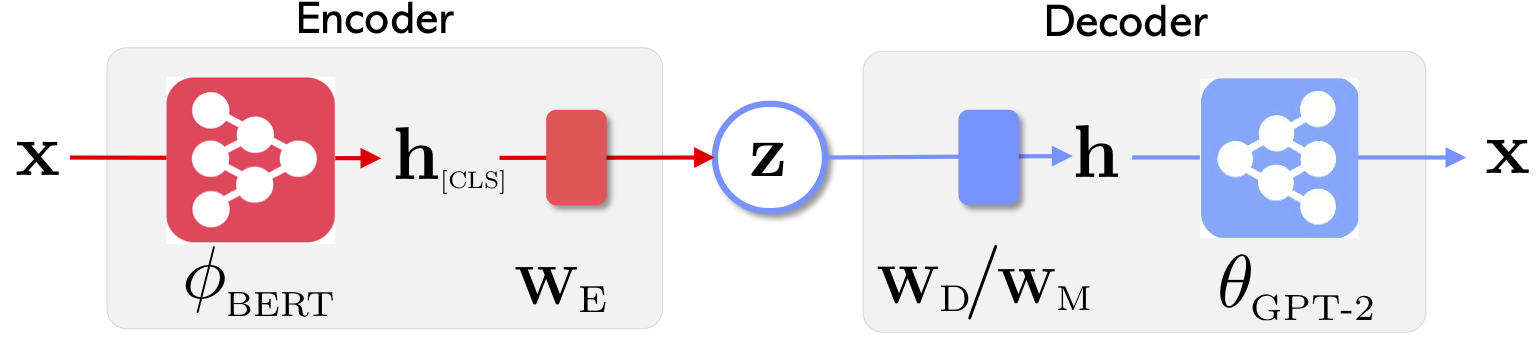
\includegraphics[width=\textwidth]{bilder/optimus_scheme}
\end{figure}

% BERT und GPT-2 über eine VAE Architektur miteinander zu verbinden hat die Herausforderung, die unterschiedlichen Tokenisierungsschemen der einzelnen Modelle zu verwenden und den Latentvektor bei der Textgeneration von GPT-2 zu injizieren. 
% Die Eingabetokens von BERT verwenden das WordPiece Embedding Verfahren \citep{wordpiece} mit einer Vokabulargröße von 28.996 Tokens. 
% Die Ausgabe erfolgt über die Byte Pair Encoding Tokenisierung \citep{bytepairencoding} von GPT-2 mit einer Vokabulargröße von 50.260 Tokens. 
% Innerhalb des Netzwerkes wird im Latentvektor ein Token durch eine Einbettung $h_{Emb}$, die das Token, die Position und das Segment Embedding wiedergibt, repräsentiert.
% Um beim Training den Loss der Rekonstruktionsaufgabe zu berechnen, werden die Sätze mit beiden Tokenisierungen tokenisiert.


% Als Latentvektor $z \in \mathbb{R}^P$ wird die gepoolte Ausgabe des letzten Hiddenlayers $h_{[CLS]} \in \mathbb{R}^H$ von BERT mit einer Gewichtsmatrix multipliziert $W_{E} \in \mathbb{R}^{P\times H}$ gewählt. Somit kann ein Latentvektor wie folgt bestimmt werden $z = W_{E}h_{[CLS]}$.

\end{frame}

\begin{frame}{Optimus}
  \begin{itemize}
    \item BERT und GPT-2 haben unterschiedliche Tokenisierungen $\Rightarrow$ beide benutzen 
    \item Latentvektor $z \in \mathbb{R}^P$ ist gepoolte Ausgabe des letzten Hiddenlayers $h_{[CLS]} \in \mathbb{R}^H$ von BERT mit einer Gewichtsmatrix multipliziert $W_{E} \in \mathbb{R}^{P\times H}$ gewählt $\Rightarrow$ $z = W_{E}h_{[CLS]}$.
  \end{itemize}

  \begin{figure}[h]
    \centering
    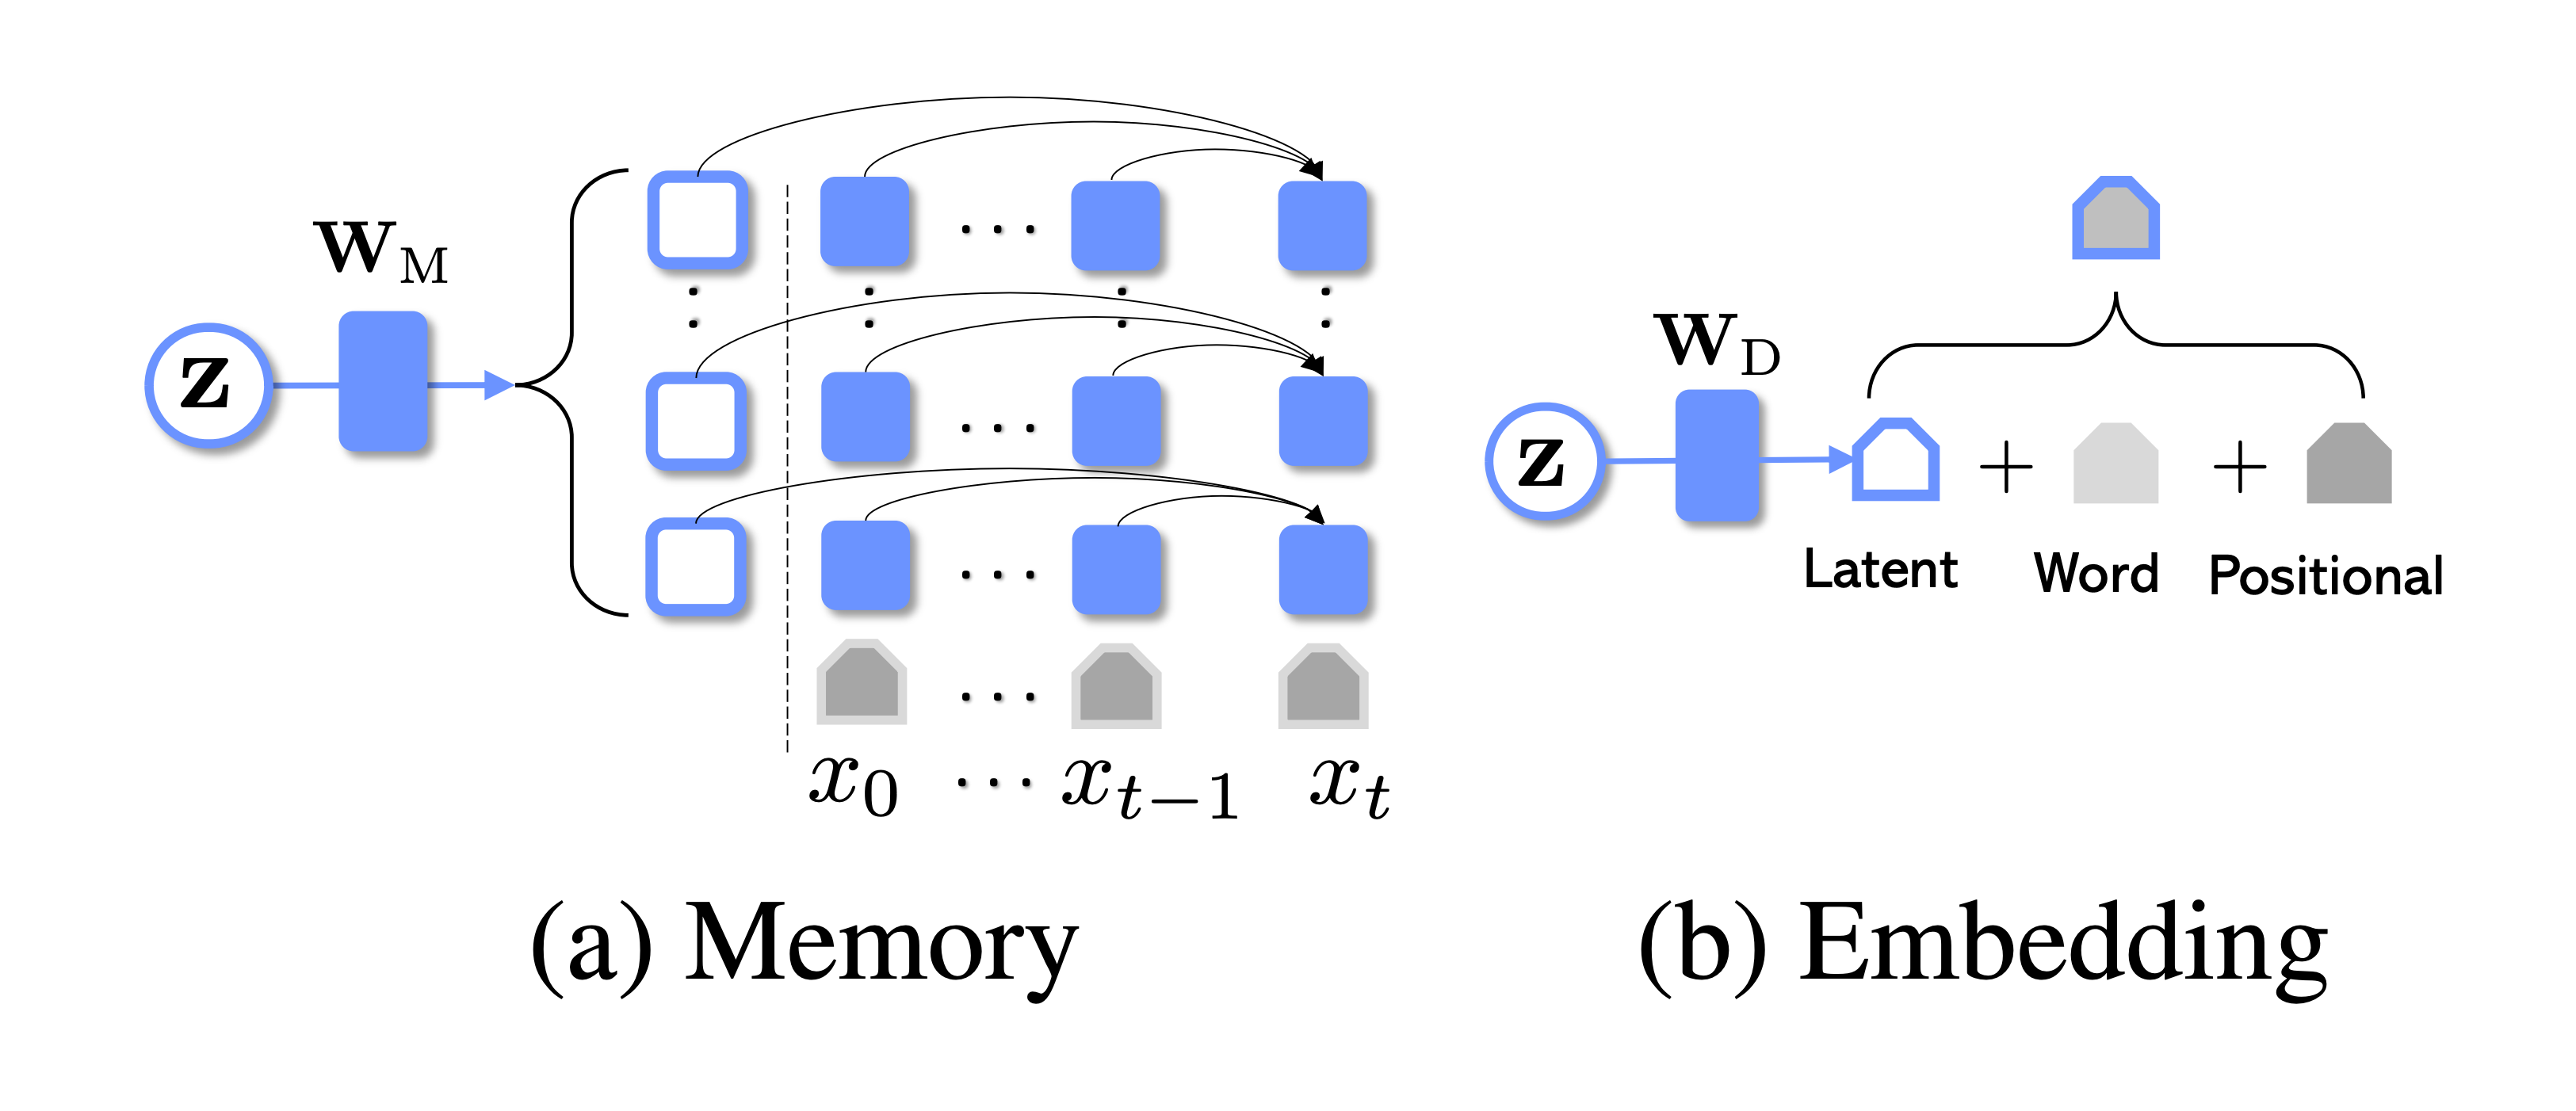
\includegraphics[width=11cm]{bilder/latent_optimus}
\end{figure}

\end{frame}

\begin{frame}{\textsc{BiMeanVAE}}
 \begin{itemize}
\item Bidirektionaler LSTM Encoder (anschließend Mean Pooling Layer)
\item LSTM Decoder
\item Hiddensize 512
\item trainiert mit Cyclical Annealing Verfahren
 \end{itemize}
\end{frame}

%MORE GRUNDLAGEN